\documentclass[a4paper, 12pt]{article}
\usepackage{listings}
\usepackage{color}
\usepackage[latin1]{inputenc}
\usepackage[T1]{fontenc}
\usepackage{graphicx}
\usepackage[]{algorithm2e}
\definecolor{deepblue}{rgb}{0,0.5,0.8}
\definecolor{dkgreen}{rgb}{0,0.6,0}
\definecolor{gray}{rgb}{0.5,0.5,0.5}
\definecolor{mauve}{rgb}{0.58,0,0.82}

\lstset{
  otherkeywords={},
  language = python,
  aboveskip = 2mm,
  belowskip = 2mm,
  showstringspaces = false,
  columns = flexible,
  basicstyle = {\small\ttfamily},
  numbers = none,			% def = left
  numberstyle = \small\color{gray},
  breaklines = false,			%scelgo se troncare le righe o meno
  breakatwhitespace = true,
  tabsize = 3,
  emph = {True, False, return},          
  emphstyle=\color{mauve},   
}

\begin{document}
\begin{center}
\LARGE\textbf{TVPR: Top View Person Re-identification}\\
\vspace{1em}
\small{Adel Massimo Ramadan, adel.massimo.ramadan@gmail.com\\
Riccardo Reali, finokkio@gmail.com\\
Ciolini Alberto, albeciolo@stud.unifi.it}\\
\vspace{0.75em}
X agosto 2017
\end{center}
\begin{center}
\end{center}

\tableofcontents
\newpage

\section{Introduzione}		%----------------------- Introduzione-------------------------------------------------------------------------------
Un importante compito per sistemi muti-camera distribuiti � il riconoscimento di un individuo in scene diverse, a tempi diversi: questo � noto come problema di \emph{Person Re-identification}.\\
La Person Re-identification � un'importante disciplina di settori come \emph{Human Computer Interaction},  \emph{Screen Monitoring}, \emph{Ambient Assisted Living} e molti altri rami di ricerca della \emph{Computer Vision}.
Si possono avere casi d'uso \emph{Online} o \emph{Offline}: nel primo caso l'analisi sul soggetto � immediata; mentre nel secondo caso si analizza la scena in differita (spesso avendo a disposizione una quantit� di informazioni maggiore).\\
Nel caso studiato il contesto � quello di un sistema offline, basato su un sistema di \emph{depht cameras}\footnote{Asus Xtion Pro Live | \href{https://www.asus.com/3D-Sensor}}: le osservazioni di questo sistema vanno a comporre il dataset \emph{TVPR}\footnote{Universit� Politecnica delle Marche: \href{http://vrai.dii.univpm.it/re-id-dataset}}. In questo dataset sono presenti 23 video, ognuno nel formato 640x480, a un frame rate prossimo a 30fps, e disponibile in formato non compresso (\emph{.ONI}); in questi video compaiono 100 persone nel loro normale modo di fare quotidiano.

\section{Obiettivi}        %----------------------- Obiettivi-------------------------------------------------------------------------------
Il principale obiettivo di questo progetto consiste nella realizzazione di un sistema in grado di stabilire se, dato un soggetto osservato al tempo $t_{0}$, questo sia presente o meno in un altra osservazione effettuata al tempo $t_{1}$.
\begin{center}
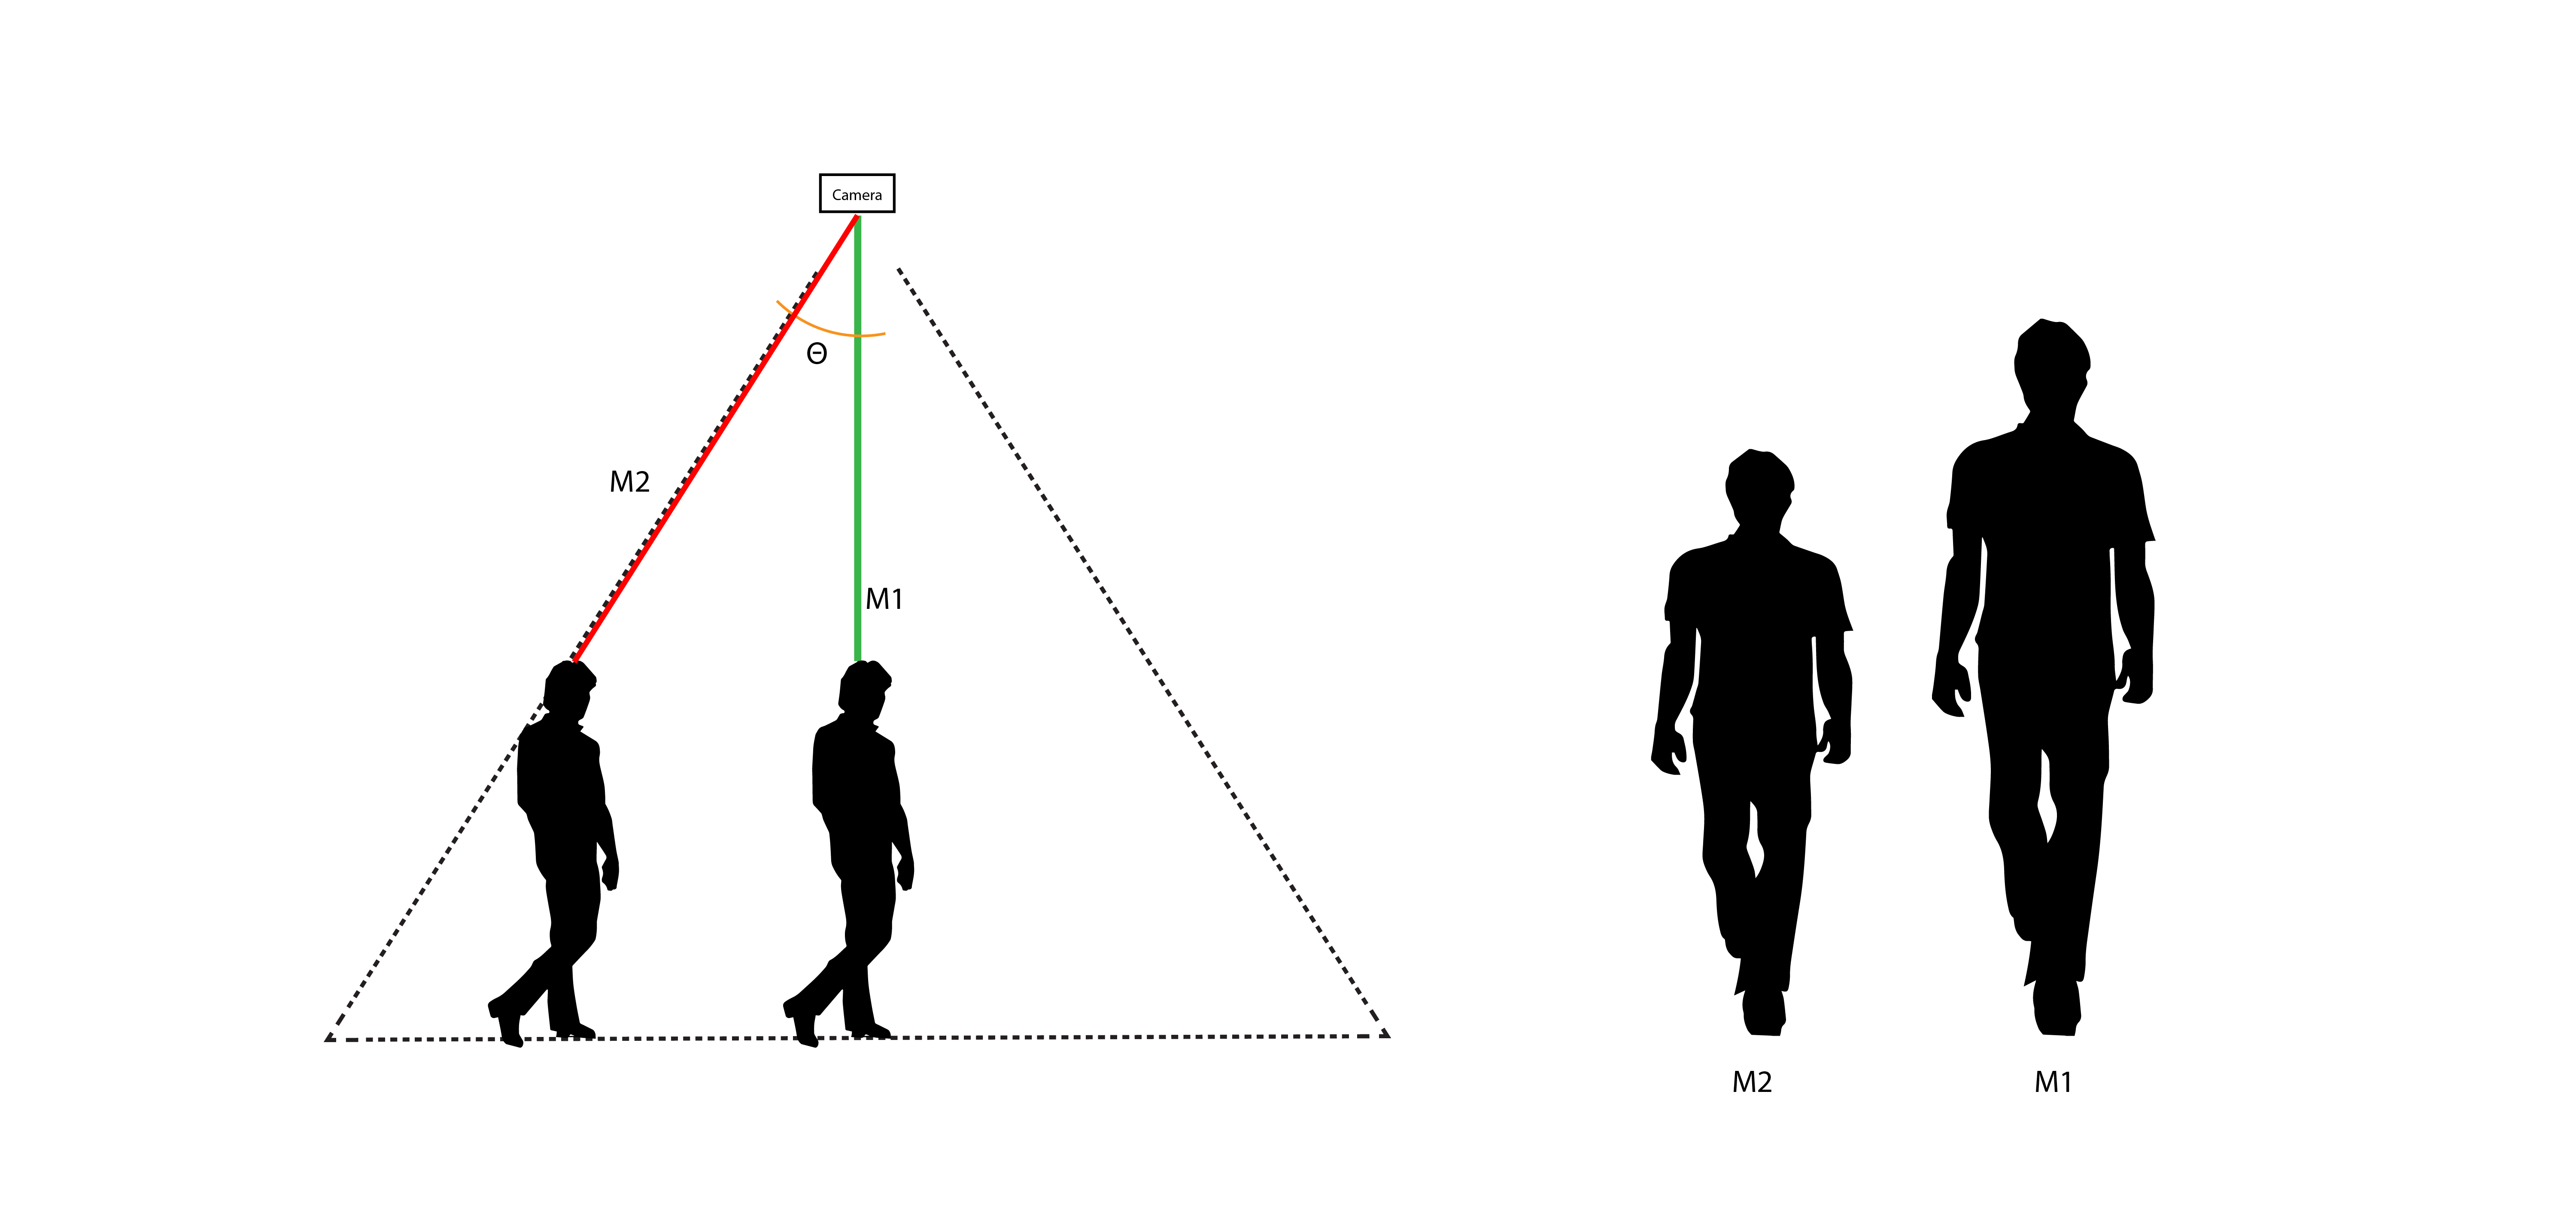
\includegraphics[scale=0.1]{immagini/img-01.png}
\end{center}
\begin{figure}
\centering
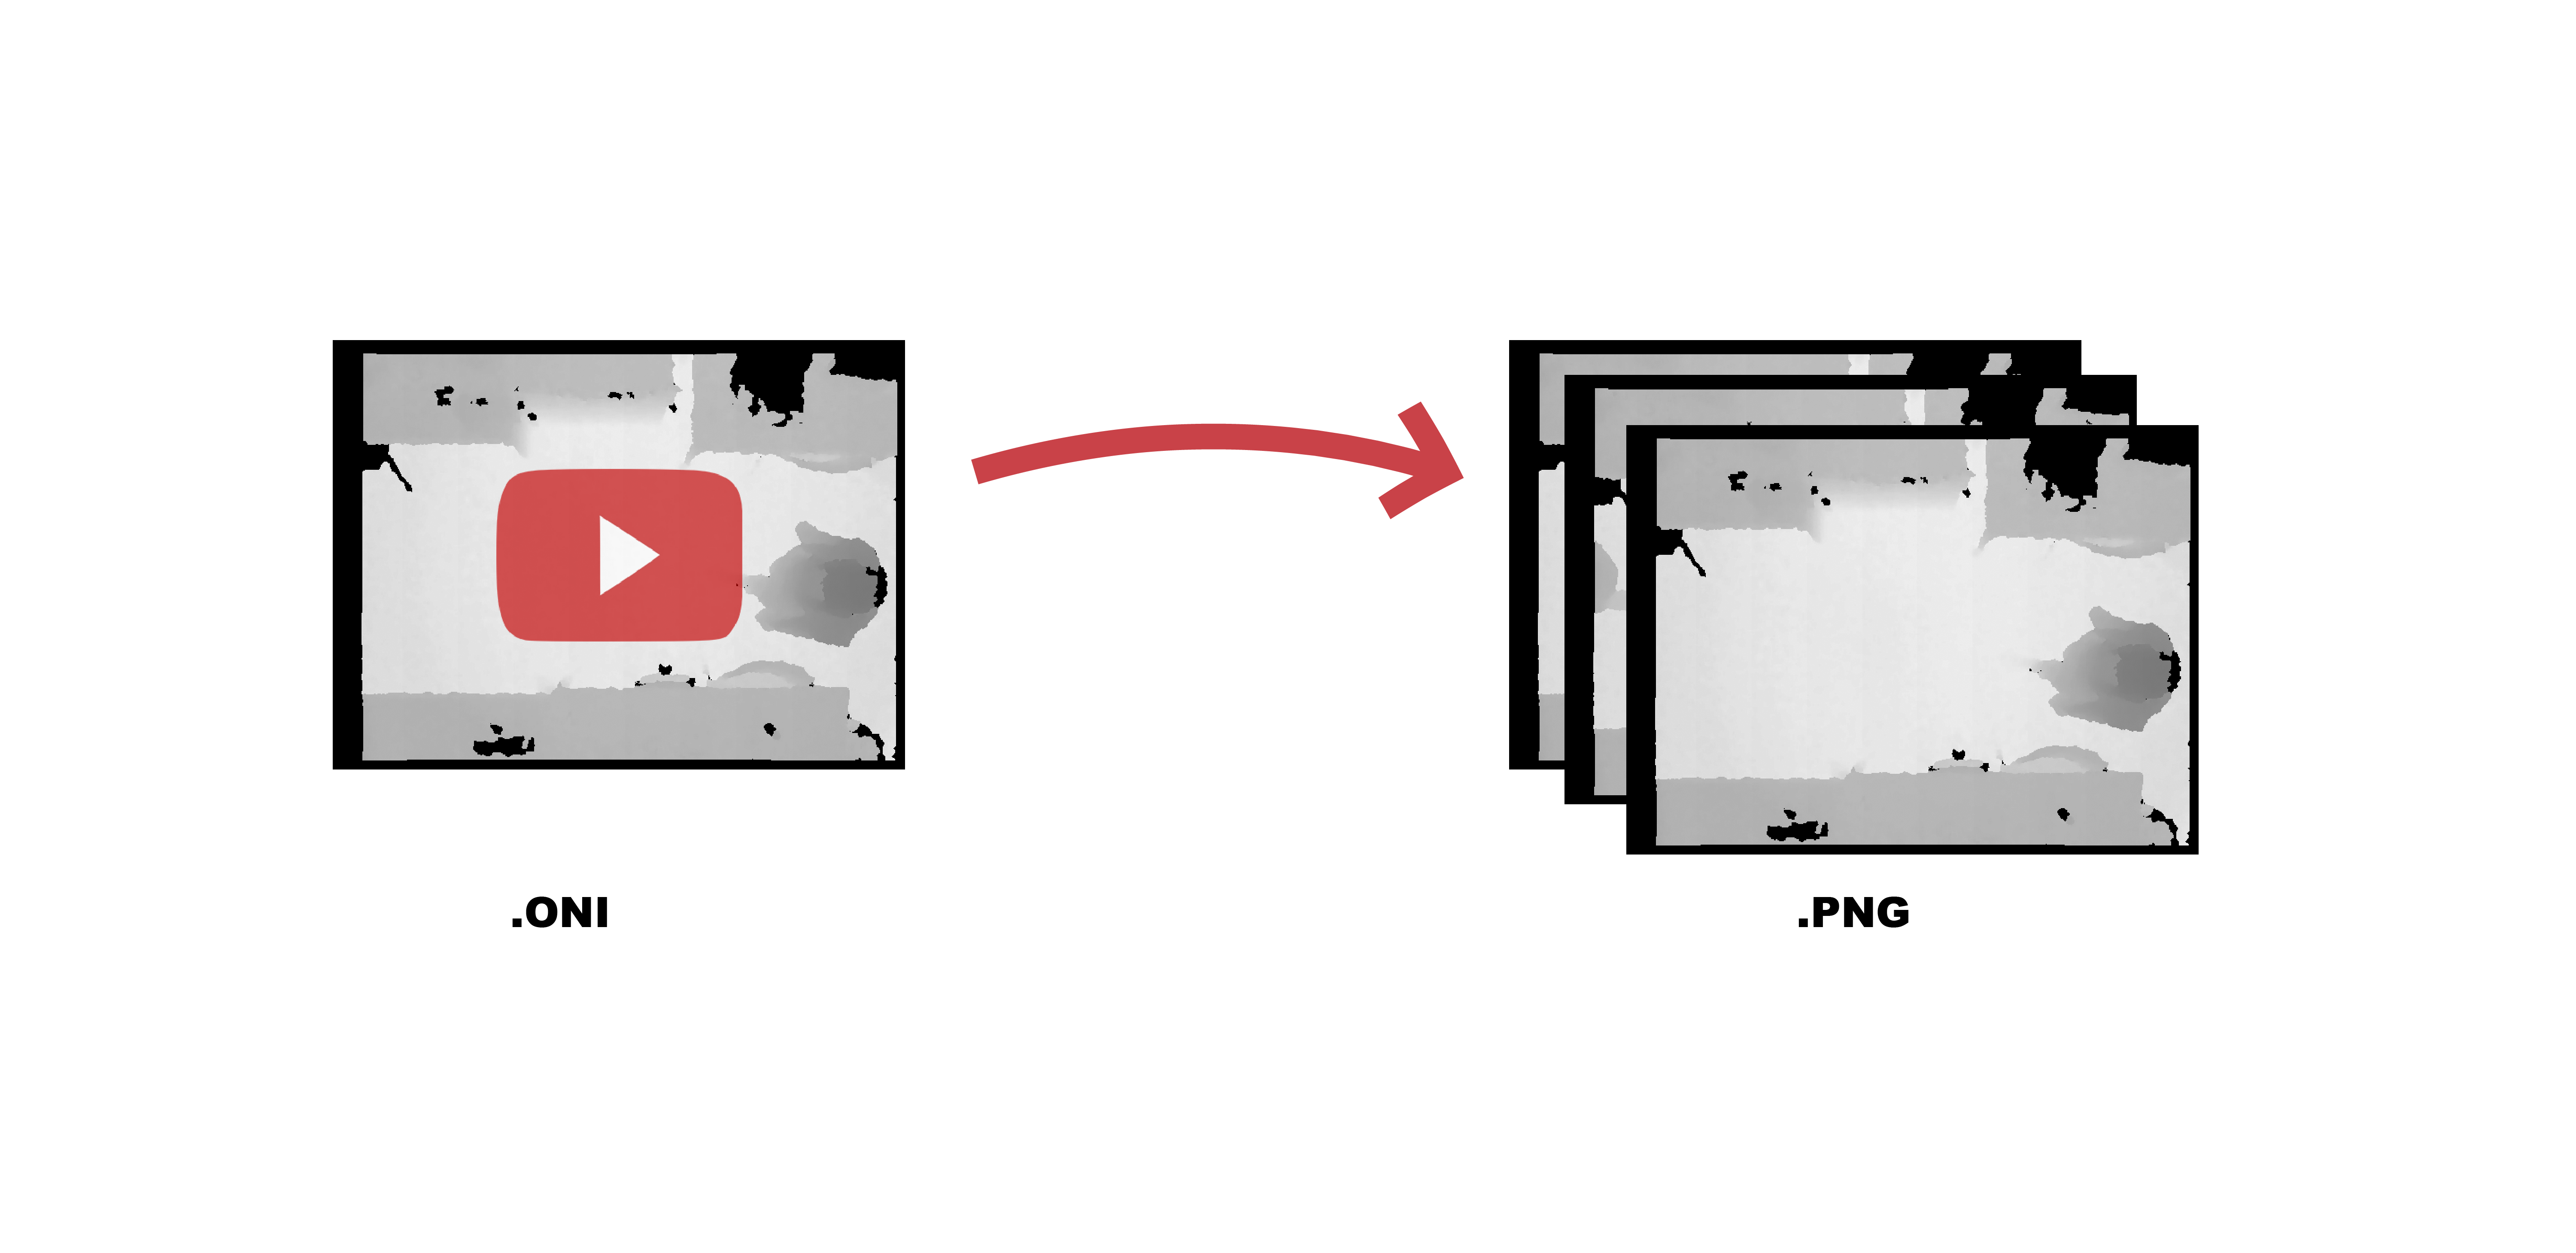
\includegraphics[scale=0.1]{immagini/img-02.png}
\caption{Il primo mockup dell'estensione}
\end{figure}

\end{document}